\documentclass[11pt,a4paper]{report}
\usepackage[textwidth=37em,vmargin=30mm]{geometry}
\usepackage{calc,xunicode,amsmath,amssymb,paralist,enumitem,tabu,booktabs,datetime2,xeCJK,xeCJKfntef,listings}
\usepackage{tocloft,fancyhdr,tcolorbox,xcolor,graphicx,eso-pic,xltxtra,xelatexemoji}

\newcommand{\envyear}[0]{2025}
\newcommand{\envdatestr}[0]{2025-01-25}
\newcommand{\envfinaldir}[0]{webdb/2025/20250125/final}

\usepackage[hidelinks]{hyperref}
\hypersetup{
    colorlinks=false,
    pdfpagemode=FullScreen,
    pdftitle={Web Digest - \envdatestr}
}

\setlength{\cftbeforechapskip}{10pt}
\renewcommand{\cftchapfont}{\rmfamily\bfseries\large\raggedright}
\setlength{\cftbeforesecskip}{2pt}
\renewcommand{\cftsecfont}{\sffamily\small\raggedright}

\setdefaultleftmargin{2em}{2em}{1em}{1em}{1em}{1em}

\usepackage{xeCJK,xeCJKfntef}
\xeCJKsetup{PunctStyle=plain,RubberPunctSkip=false,CJKglue=\strut\hskip 0pt plus 0.1em minus 0.05em,CJKecglue=\strut\hskip 0.22em plus 0.2em}
\XeTeXlinebreaklocale "zh"
\XeTeXlinebreakskip = 0pt


\setmainfont{Brygada 1918}
\setromanfont{Brygada 1918}
\setsansfont{IBM Plex Sans}
\setmonofont{JetBrains Mono NL}
\setCJKmainfont{Noto Serif CJK SC}
\setCJKromanfont{Noto Serif CJK SC}
\setCJKsansfont{Noto Sans CJK SC}
\setCJKmonofont{Noto Sans CJK SC}

\setlength{\parindent}{0pt}
\setlength{\parskip}{8pt}
\linespread{1.15}

\lstset{
	basicstyle=\ttfamily\footnotesize,
	numbersep=5pt,
	backgroundcolor=\color{black!5},
	showspaces=false,
	showstringspaces=false,
	showtabs=false,
	tabsize=2,
	captionpos=b,
	breaklines=true,
	breakatwhitespace=true,
	breakautoindent=true,
	linewidth=\textwidth
}






\newcommand{\coverpic}[2]{
    % argv: itemurl, authorname
    Cover photo by #2~~(\href{#1}{#1})
}
\newcommand{\makeheader}[0]{
    \begin{titlepage}
        % \newgeometry{hmargin=15mm,tmargin=21mm,bmargin=12mm}
        \begin{center}
            
            \rmfamily\scshape
            \fontspec{BaskervilleF}
            \fontspec{Old Standard}
            \fontsize{59pt}{70pt}\selectfont
            WEB\hfill DIGEST
            
            \vfill
            % \vskip 30pt
            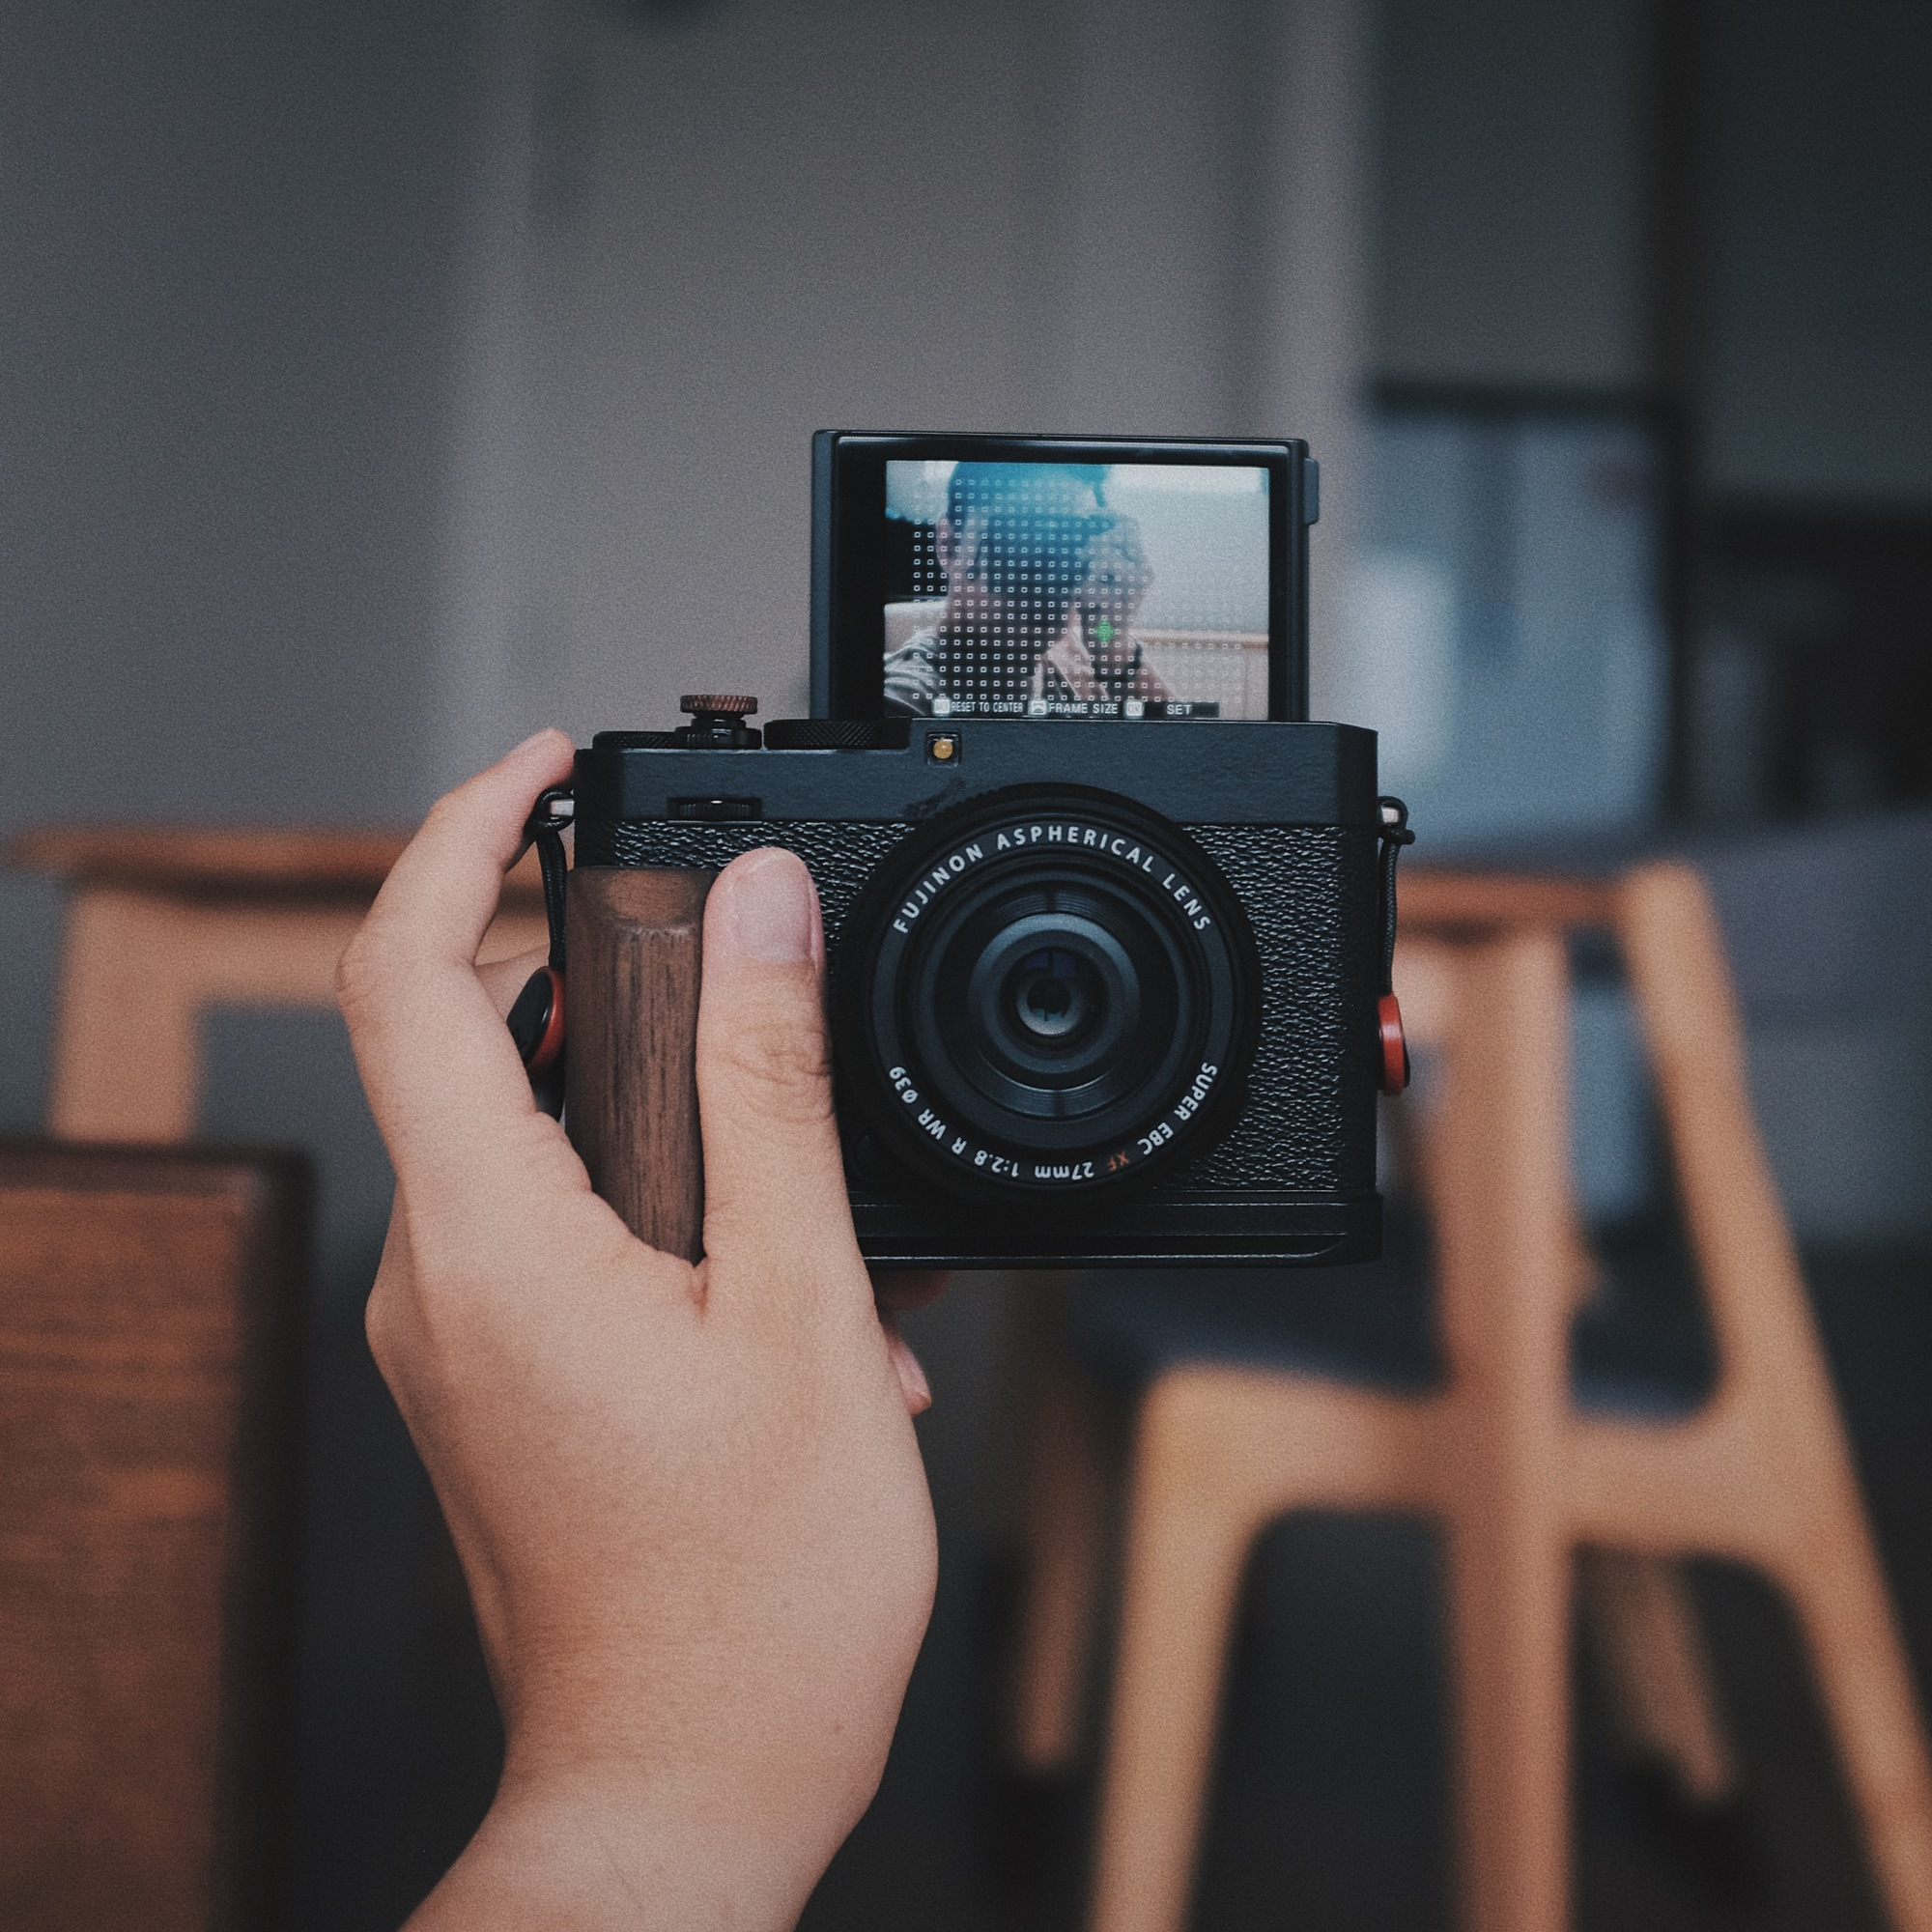
\includegraphics[width=\linewidth]{\envfinaldir/coverpic-prod.jpg}\par
            % \vskip 30pt
            \vfill

            \normalsize\rmfamily\scshape
            \copyright{} The Web Digest Project \hfill\large \envdatestr
        \end{center}
    \end{titlepage}
    % \restoregeometry
}
\newcommand{\simplehref}[1]{%
    \textcolor{blue!80!green}{\href{#1}{#1}}%
}
\renewcommand{\contentsname}{\center\Huge\sffamily\bfseries Contents\par\vskip 20pt}
\newcounter{ipartcounter}
\setcounter{ipartcounter}{0}
\newcommand{\ipart}[1]{
    % \vskip 20pt
    \clearpage
    \stepcounter{ipartcounter}
    \phantomsection
    \addcontentsline{toc}{chapter}{#1}
    % \begin{center}
    %     \Huge
    %     \sffamily\bfseries
    %     #1
    % \end{center}
    % \vskip 20pt plus 7pt
}
\newcounter{ichaptercounter}
\setcounter{ichaptercounter}{0}
\newcommand{\ichapter}[1]{
    % \vskip 20pt
    \clearpage
    \stepcounter{ichaptercounter}
    \phantomsection
    \addcontentsline{toc}{section}{\numberline{\arabic{ichaptercounter}}#1}
    \begin{center}
        \Huge
        \sffamily\bfseries
        #1
    \end{center}
    \vskip 20pt plus 7pt
}
\newcommand{\entrytitlefont}[1]{\subsection*{\raggedright\Large\sffamily\bfseries#1}}
\newcommand{\entryitemGeneric}[2]{
    % argv: title, url
    \parbox{\linewidth}{
        \entrytitlefont{#1}\par\vskip 5pt
        \footnotesize\ttfamily\mdseries
        \simplehref{#2}
    }\vskip 11pt plus 11pt minus 1pt
}
\newcommand{\entryitemGithub}[3]{
    % argv: title, url, desc
    \parbox{\linewidth}{
        \entrytitlefont{#1}\par\vskip 5pt
        \footnotesize\ttfamily\mdseries
        \simplehref{#2}\par\vskip 5pt
        \small\rmfamily\mdseries#3
    }\vskip 11pt plus 11pt minus 1pt
}
\newcommand{\entryitemAp}[3]{
    % argv: title, url, desc
    \parbox{\linewidth}{
        \entrytitlefont{#1}\par\vskip 5pt
        \footnotesize\ttfamily\mdseries
        \simplehref{#2}\par\vskip 5pt
        \small\rmfamily\mdseries#3
    }\vskip 11pt plus 11pt minus 1pt
}
\newcommand{\entryitemHackernews}[3]{
    % argv: title, hnurl, rawurl
    % \parbox{\linewidth}{
    %     \entrytitlefont{#1}\par\vskip 5pt
    %     \footnotesize\ttfamily\mdseries
    %     \simplehref{#3}\par
    %     \textcolor{black!50}{\href{#2}{#2}}
    % }\vskip 11pt plus 11pt minus 1pt
    \begin{minipage}{\linewidth}
            \entrytitlefont{#1}\par\vskip 5pt
            \footnotesize\ttfamily\mdseries
            \simplehref{#3}\par
            \textcolor{black!50}{\href{#2}{#2}}
    \end{minipage}\par\vskip 11pt plus 11pt minus 1pt
}







\begin{document}

\makeheader

\tableofcontents\clearpage




\ipart{Developers}
\ichapter{Hacker News}
\entryitemTwoLinks{PhysicsForums and the Dead Internet Theory}{https://news.ycombinator.com/item?id=42816284}{https://hallofdreams.org/posts/physicsforums/}

\entryitemTwoLinks{Subpixel Snake [video]}{https://news.ycombinator.com/item?id=42815288}{https://www.youtube.com/watch?v=iDwganLjpW0}

\entryitemTwoLinks{A WebAssembly compiler that fits in a tweet}{https://news.ycombinator.com/item?id=42814948}{https://wasmgroundup.com/blog/wasm-compiler-in-a-tweet/}

\entryitemTwoLinks{Snowdrop OS – a homebrew operating system from scratch, in assembly language}{https://news.ycombinator.com/item?id=42814820}{http://sebastianmihai.com/snowdrop/}

\entryitemTwoLinks{Wild – A fast linker for Linux}{https://news.ycombinator.com/item?id=42814683}{https://github.com/davidlattimore/wild}

\entryitemTwoLinks{New Book-Sorting Algorithm Almost Reaches Perfection}{https://news.ycombinator.com/item?id=42814275}{https://www.quantamagazine.org/new-book-sorting-algorithm-almost-reaches-perfection-20250124/}

\entryitemTwoLinks{Show HN: Cs16.css – CSS library based on Counter Strike 1.6 UI}{https://news.ycombinator.com/item?id=42814110}{https://cs16.samke.me}

\entryitemTwoLinks{How I Use Home Assistant in 2025}{https://news.ycombinator.com/item?id=42813513}{https://vpetersson.com/2025/01/22/how-i-use-home-assistant-in-2025.html}

\entryitemTwoLinks{Bluesky's science takeover: 70\% of Nature poll respondents use platform}{https://news.ycombinator.com/item?id=42813316}{https://www.nature.com/articles/d41586-025-00177-1}

\entryitemTwoLinks{Little Snitch feature nobody knows about}{https://news.ycombinator.com/item?id=42813231}{https://lapcatsoftware.com/articles/2025/1/6.html}

\entryitemTwoLinks{Every System is a Log: Avoiding coordination in distributed applications}{https://news.ycombinator.com/item?id=42813049}{https://restate.dev/blog/every-system-is-a-log-avoiding-coordination-in-distributed-applications/}

\entryitemTwoLinks{Lightpanda: Headless browser designed for AI and automation}{https://news.ycombinator.com/item?id=42812859}{https://github.com/lightpanda-io/browser}

\entryitemTwoLinks{Ask HN: Why buy domains and 301 redirect them to me?}{https://news.ycombinator.com/item?id=42812779}{https://news.ycombinator.com/item?id=42812779}

\entryitemTwoLinks{Build It Yourself}{https://news.ycombinator.com/item?id=42812641}{https://lucumr.pocoo.org/2025/1/24/build-it-yourself/}

\entryitemTwoLinks{We Need to Talk About Docker Hub}{https://news.ycombinator.com/item?id=42812203}{https://www.linuxserver.io/blog/we-need-to-talk-about-docker-hub}

\entryitemTwoLinks{UI is hell: four-function calculators}{https://news.ycombinator.com/item?id=42810300}{https://lcamtuf.substack.com/p/ui-is-hell-four-function-calculators}

\entryitemTwoLinks{A phishing attack involving g.co, Google's URL shortener}{https://news.ycombinator.com/item?id=42810252}{https://gist.github.com/zachlatta/f86317493654b550c689dc6509973aa4}

\entryitemTwoLinks{The State of Vim}{https://news.ycombinator.com/item?id=42810176}{https://lwn.net/Articles/1002342/}

\entryitemTwoLinks{AI isn't going to kill the software industry}{https://news.ycombinator.com/item?id=42810175}{https://dustinewers.com/ignore-the-grifters/}

\entryitemTwoLinks{Weierstrass's Monster}{https://news.ycombinator.com/item?id=42810103}{https://www.quantamagazine.org/the-jagged-monstrous-function-that-broke-calculus-20250123/}\ichapter{Phoronix}
\entryitemGeneric{\hskip 0pt{}Linux 6.14 Adds Support For Blaize BLZP1600, SpacemiT K1 \& Snapdragon 8 Elite SoCs}{https://www.phoronix.com/news/Linux-6.14-SoCs}

\entryitemGeneric{\hskip 0pt{}Vulkan 1.4.306 Published With Two More Extensions}{https://www.phoronix.com/news/Vulkan-1.4.306}

\entryitemGeneric{\hskip 0pt{}NVIDIA GeForce RTX 5090 Linux GPU Compute Performance Benchmarks}{https://www.phoronix.com/review/nvidia-geforce-rtx5090-linux}

\entryitemGeneric{\hskip 0pt{}Several Linux DRM Drivers Orphaned Due To Developer Health}{https://www.phoronix.com/news/Several-Linux-DRM-Orphaned}

\entryitemGeneric{\hskip 0pt{}Linux 6.14 Delivering Better Read Performance For CIFS}{https://www.phoronix.com/news/Linux-6.14-Faster-CIFS-Reads}

\entryitemGeneric{\hskip 0pt{}GNOME Showtime Video Player Won't Be Ready Until GNOME 49}{https://www.phoronix.com/news/GNOME-49-Showtime-Plan}

\entryitemGeneric{\hskip 0pt{}XFS Code For Linux 6.14 Improves Realtime Device Support}{https://www.phoronix.com/news/Linux-6.14-XFS}

\entryitemGeneric{\hskip 0pt{}NVIDIA Maxwell, Pascal \& Volta Support Looks Like It Will Soon Move To A Legacy Driver}{https://www.phoronix.com/news/Maxwe--Pascal-Volta-Legacy-Near}

\entryitemGeneric{\hskip 0pt{}Fedora Preparing For A Data Center Move For More Power \& Space For Possible RISC-V}{https://www.phoronix.com/news/Fedora-2024-Data-Center-Move}\ichapter{Dribbble}
\entryitemGeneric{\hskip 0pt{}Tattooed Devil Horns}{https://dribbble.com/shots/25520911-Tattooed-Devil-Horns}

\entryitemGeneric{\hskip 0pt{}Carbon Solutions B2B Dashboard Design}{https://dribbble.com/shots/25506638-Carbon-Solutions-B2B-Dashboard-Design}

\entryitemGeneric{\hskip 0pt{}Rapid Rabbit Logo}{https://dribbble.com/shots/25516738-Rapid-Rabbit-Logo}

\entryitemGeneric{\hskip 0pt{}Goose Gym}{https://dribbble.com/shots/25515121-Goose-Gym}

\entryitemGeneric{\hskip 0pt{}VCC Unused Logo Design Concept}{https://dribbble.com/shots/25511334-VCC-Unused-Logo-Design-Concept}

\entryitemGeneric{\hskip 0pt{}HappyDev - Logo Design / Branding}{https://dribbble.com/shots/25514894-HappyDev-Logo-Design-Branding}

\entryitemGeneric{\hskip 0pt{}LLM GPU Manager}{https://dribbble.com/shots/25513811-LLM-GPU-Manager}

\entryitemGeneric{\hskip 0pt{}Product design - icons set}{https://dribbble.com/shots/25516253-Product-design-icons-set}

\entryitemGeneric{\hskip 0pt{}The Toucan}{https://dribbble.com/shots/25515890-The-Toucan}

\entryitemGeneric{\hskip 0pt{}Bestest Brand®}{https://dribbble.com/shots/25510300-Bestest-Brand}

\entryitemGeneric{\hskip 0pt{}QVELTY / Design \& Animation}{https://dribbble.com/shots/25507639-QVELTY-Design-Animation}

\entryitemGeneric{\hskip 0pt{}Wine Label}{https://dribbble.com/shots/25509757-Wine-Label}

\entryitemGeneric{\hskip 0pt{}Haptic Logo Design}{https://dribbble.com/shots/25504012-Haptic-Logo-Design}

\entryitemGeneric{\hskip 0pt{}Letter V + LED + Wires Logo}{https://dribbble.com/shots/25507506-Letter-V-LED-Wires-Logo}

\entryitemGeneric{\hskip 0pt{}Robin bird logo}{https://dribbble.com/shots/25509208-Robin-bird-logo}

\entryitemGeneric{\hskip 0pt{}Qore - Logo Design}{https://dribbble.com/shots/25509466-Qore-Logo-Design}

\entryitemGeneric{\hskip 0pt{}Wine Label}{https://dribbble.com/shots/25503830-Wine-Label}

\entryitemGeneric{\hskip 0pt{}Monocle Cat}{https://dribbble.com/shots/25502155-Monocle-Cat}

\entryitemGeneric{\hskip 0pt{}Roundrobin}{https://dribbble.com/shots/25502404-Roundrobin}

\entryitemGeneric{\hskip 0pt{}Mobile Game Design}{https://dribbble.com/shots/25498605-Mobile-Game-Design}

\entryitemGeneric{\hskip 0pt{}"Nature Morte" - Promotional piece}{https://dribbble.com/shots/25501105--Nature-Morte-Promotional-piece}

\entryitemGeneric{\hskip 0pt{}Fitness App Design}{https://dribbble.com/shots/25494068-Fitness-App-Design}

\entryitemGeneric{\hskip 0pt{}404}{https://dribbble.com/shots/25492419-404}

\entryitemGeneric{\hskip 0pt{}Personal Banking App}{https://dribbble.com/shots/25493958-Personal-Banking-App}


\ipart{Developers~~~~(zh-Hans)}
\ichapter{Solidot}
\entryitemGeneric{\hskip 0pt{}调查显示八成游戏开发商开发 PC 游戏}{https://www.solidot.org/story?sid=80418}

\entryitemGeneric{\hskip 0pt{}《自然》调查显示七成回应者使用 Bluesky}{https://www.solidot.org/story?sid=80417}

\entryitemGeneric{\hskip 0pt{}乔治 R.R.马丁合作发表了一篇物理学论文}{https://www.solidot.org/story?sid=80416}

\entryitemGeneric{\hskip 0pt{}Google 移动搜索移除网址面包屑导航}{https://www.solidot.org/story?sid=80415}

\entryitemGeneric{\hskip 0pt{}癌细胞利用有缺陷的线粒体毒害攻击免疫细胞}{https://www.solidot.org/story?sid=80414}

\entryitemGeneric{\hskip 0pt{}日本市场中国平板电视首次超过五成}{https://www.solidot.org/story?sid=80413}

\entryitemGeneric{\hskip 0pt{}智人离开非洲后血型可能发生适应性遗传变化}{https://www.solidot.org/story?sid=80412}

\entryitemGeneric{\hskip 0pt{}三菱不打算参与本田日产的合并}{https://www.solidot.org/story?sid=80411}

\entryitemGeneric{\hskip 0pt{}特朗普政府暂停了 NIH 的会议和旅行}{https://www.solidot.org/story?sid=80410}

\entryitemGeneric{\hskip 0pt{}Debian 15 代号 Duke}{https://www.solidot.org/story?sid=80409}

\entryitemGeneric{\hskip 0pt{}研究揭示不同政治光谱对传递虚假信息的偏好}{https://www.solidot.org/story?sid=80408}

\entryitemGeneric{\hskip 0pt{}万事达卡 DNS 错误存在了五年之久}{https://www.solidot.org/story?sid=80405}

\entryitemGeneric{\hskip 0pt{}Debian 13.0 Trixie 预计今年夏天发布}{https://www.solidot.org/story?sid=80404}

\entryitemGeneric{\hskip 0pt{}Telegram 屏蔽 RuTracker 频道}{https://www.solidot.org/story?sid=80402}

\entryitemGeneric{\hskip 0pt{}在出售给美国买家前苹果应用商店不会重新上架 TikTok}{https://www.solidot.org/story?sid=80400}

\entryitemGeneric{\hskip 0pt{}过去一个世纪男性身高体重增长速度两倍于女性}{https://www.solidot.org/story?sid=80399}

\entryitemGeneric{\hskip 0pt{}杭州深度求索发布能挑战 OpenAI o1 的推理模型 DeepSeek R1}{https://www.solidot.org/story?sid=80398}

\entryitemGeneric{\hskip 0pt{}黑猩猩的撒尿行为具有传染性}{https://www.solidot.org/story?sid=80397}

\entryitemGeneric{\hskip 0pt{}耐药菌在乌克兰扩散}{https://www.solidot.org/story?sid=80396}

\entryitemGeneric{\hskip 0pt{}中国 2024 年可更新能源装机容量再创记录}{https://www.solidot.org/story?sid=80395}\ichapter{V2EX}
\entryitemGeneric{\hskip 0pt{}[macOS] Raycast 搜索文件总是不全,始终 indexing files 或者 indexing error。请大佬支招}{https://www.v2ex.com/t/1107736}

\entryitemGeneric{\hskip 0pt{}[iPhone] 有替代 simbox 的多卡待机解决方案吗?}{https://www.v2ex.com/t/1107735}

\entryitemGeneric{\hskip 0pt{}[分享创造] 为小红书和 TikTok 创作者打造的全新平台,帮助 TikTok 博主顺利转型至 Rednote,助力内容创作!}{https://www.v2ex.com/t/1107734}

\entryitemGeneric{\hskip 0pt{}[问与答] 用 C\#搓了个小工具,但有个诡异的地方不知如何解决}{https://www.v2ex.com/t/1107733}

\entryitemGeneric{\hskip 0pt{}[问与答] VSCode Remote-SSH Server 下载速度巨慢怎么办?}{https://www.v2ex.com/t/1107731}

\entryitemGeneric{\hskip 0pt{}[分享创造] 魔改了一下 cool retro term 终端,增加了 AI 的侧边栏,开源可下载}{https://www.v2ex.com/t/1107729}

\entryitemGeneric{\hskip 0pt{}[程序员] XXL-CONF v1.7.0 | 分布式服务管理平台(配置中心 \& 注册中心)}{https://www.v2ex.com/t/1107728}

\entryitemGeneric{\hskip 0pt{}[Kubernetes] 各位工作的公司生产 k8s 是怎么维护应用的 request 和 limit 的?}{https://www.v2ex.com/t/1107726}

\entryitemGeneric{\hskip 0pt{}[分享发现] 求推荐合适的 NAS 机箱}{https://www.v2ex.com/t/1107725}

\entryitemGeneric{\hskip 0pt{}[分享创造] 千呼万唤使出来, AI 换脸达摩神器 PicMagix 终于上线了!}{https://www.v2ex.com/t/1107724}

\entryitemGeneric{\hskip 0pt{}[问与答] 一个笔记产品 Affine}{https://www.v2ex.com/t/1107723}

\entryitemGeneric{\hskip 0pt{}[问与答] [父母医保]}{https://www.v2ex.com/t/1107722}

\entryitemGeneric{\hskip 0pt{}[Rust] Rust 编写的高性能 HTTP/HTTPS/SOCKS5 代理服务器}{https://www.v2ex.com/t/1107721}

\entryitemGeneric{\hskip 0pt{}[问与答] 各位,有什么好的手机壁纸推荐吗?}{https://www.v2ex.com/t/1107720}

\entryitemGeneric{\hskip 0pt{}[SSL] 免费赠送 10 个一年通配符域证书,通配符域证书低至\$10/年}{https://www.v2ex.com/t/1107718}

\entryitemGeneric{\hskip 0pt{}[程序员] 研究了两个月 cursor,看样子还是 cursor 不赚钱,不是活菩萨。}{https://www.v2ex.com/t/1107716}

\entryitemGeneric{\hskip 0pt{}[问与答] 12306 怎么提高抢票机率哦}{https://www.v2ex.com/t/1107715}

\entryitemGeneric{\hskip 0pt{}[问与答] 自建 dns 方案求推荐。}{https://www.v2ex.com/t/1107714}

\entryitemGeneric{\hskip 0pt{}[软件] Win11 有什么网络接口流量统计绿色软件好用?}{https://www.v2ex.com/t/1107713}

\entryitemGeneric{\hskip 0pt{}[问与答] 2025 年了,求推荐一个 MacBook pro 鼠标}{https://www.v2ex.com/t/1107712}

\entryitemGeneric{\hskip 0pt{}[NAS] 请教极空间 NAS 相册自动备份问题}{https://www.v2ex.com/t/1107711}

\entryitemGeneric{\hskip 0pt{}[问与答] Windows chrome 网页中任意文字位置可以被鼠标点击出现输入框,这是为什么?}{https://www.v2ex.com/t/1107710}

\entryitemGeneric{\hskip 0pt{}[全球工单系统] 京东 App 无视用户选择的扣款顺序,强行默认打白条支付}{https://www.v2ex.com/t/1107709}

\entryitemGeneric{\hskip 0pt{}[问与答] 苹果账号转到美国区后,抖音 App 无法更新了?}{https://www.v2ex.com/t/1107707}

\entryitemGeneric{\hskip 0pt{}[Apple] 请问妙控板可以在 2 台或多台设备间快速切换吗?}{https://www.v2ex.com/t/1107706}

\entryitemGeneric{\hskip 0pt{}[Apple] 2025 年还能买 M2 Mac mini 么?}{https://www.v2ex.com/t/1107705}

\entryitemGeneric{\hskip 0pt{}[NAS] 是 B550 芯片组不支持还是 Ryzen G 系列不支持 acs}{https://www.v2ex.com/t/1107704}

\entryitemGeneric{\hskip 0pt{}[VPS] 白嫖的 Azure B1s 主机在香港 1 区遭遇的负载拉满问题}{https://www.v2ex.com/t/1107703}

\entryitemGeneric{\hskip 0pt{}[问与答] 通过改键拯救小拇指}{https://www.v2ex.com/t/1107702}

\entryitemGeneric{\hskip 0pt{}[问与答] 哪款 4K 以上显示器有优美的白色、四边等宽边框}{https://www.v2ex.com/t/1107700}

\entryitemGeneric{\hskip 0pt{}[推广] GoSSL 在这里赠送 10 个一年通配符域证书,通配符域证书低至\$10/年}{https://www.v2ex.com/t/1107699}

\entryitemGeneric{\hskip 0pt{}[Apple] Steam 不支持 macOS Catalina 了}{https://www.v2ex.com/t/1107698}

\entryitemGeneric{\hskip 0pt{}[奇思妙想] ChatGPT 出来这么久了,怎么没看到融合实体娃娃 / 机器人的产品?}{https://www.v2ex.com/t/1107697}

\entryitemGeneric{\hskip 0pt{}[全球工单系统] B 站直播页网页全屏模式在 Safari 浏览器中两侧存在黑边}{https://www.v2ex.com/t/1107696}

\entryitemGeneric{\hskip 0pt{}[职场话题] 看来要被优化了}{https://www.v2ex.com/t/1107695}

\entryitemGeneric{\hskip 0pt{}[随想] 关于程序员找对象这事,真心有需要可以咨询/了解下~~}{https://www.v2ex.com/t/1107694}

\entryitemGeneric{\hskip 0pt{}[分享发现] \# AIFly.Tools - 全球化的 AI 工具发现平台}{https://www.v2ex.com/t/1107693}

\entryitemGeneric{\hskip 0pt{}[问与答] 闪迪的固态硬盘掉盘啥问题?}{https://www.v2ex.com/t/1107692}

\entryitemGeneric{\hskip 0pt{}[分享创造] 做了一个简单的红包封面, 感兴趣的话可以领取}{https://www.v2ex.com/t/1107689}

\entryitemGeneric{\hskip 0pt{}[加密货币] 用 U 理财赚的钱可以拿来买房吗?}{https://www.v2ex.com/t/1107688}

\entryitemGeneric{\hskip 0pt{}[生活] 来新公司的第一年领了两个月的年终奖}{https://www.v2ex.com/t/1107687}

\entryitemGeneric{\hskip 0pt{}[问与答] 大家每年过年还会买新衣新鞋换新装吗,可以的话,方便透露下自己的年龄区间吗,如 25~30 这样}{https://www.v2ex.com/t/1107686}

\entryitemGeneric{\hskip 0pt{}[分享创造] typecho 插件:将 Typecho 文章同步到 Notion}{https://www.v2ex.com/t/1107685}

\entryitemGeneric{\hskip 0pt{}[问与答] 大佬们, 问一下有没有画图比较专业一点的 AI}{https://www.v2ex.com/t/1107684}

\entryitemGeneric{\hskip 0pt{}[生活] 这几天开车从江浙沪往安徽方向,堵的怎么样?}{https://www.v2ex.com/t/1107682}

\entryitemGeneric{\hskip 0pt{}[问与答] 同一个 epub 电子书文件,在软件 A 上是横排,软件 B 上是竖排,为何如此?}{https://www.v2ex.com/t/1107681}

\entryitemGeneric{\hskip 0pt{}[程序员] openai 投资的 Heyboss(给不会写代码的人的 AI eng)招聘全栈月薪 3-4w}{https://www.v2ex.com/t/1107680}

\entryitemGeneric{\hskip 0pt{}[程序员] 反思:不小心伤害到了组员的自尊}{https://www.v2ex.com/t/1107679}

\entryitemGeneric{\hskip 0pt{}[淘宝] 感觉网上买的开心果都是陈货,有没有推荐的店铺}{https://www.v2ex.com/t/1107678}

\entryitemGeneric{\hskip 0pt{}[程序员] 马上下班,回家过年!}{https://www.v2ex.com/t/1107677}


\ipart{Generic News}







\clearpage
\leavevmode\vfill
\footnotesize

Copyright \copyright{} 2023-2025 Neruthes and other contributors.

This document is published with CC BY-NC-ND 4.0 license.

The entries listed in this newsletter may be copyrighted by their respective creators.

This newsletter is generated by the Web Digest project.

The newsletters are also delivered via Telegram channel \CJKunderline{\href{https://t.me/webdigestchannel}{https://t.me/webdigestchannel}}.\\
RSS feed is available at \CJKunderline{\href{https://webdigest.pages.dev/rss.xml}{https://webdigest.pages.dev/rss.xml}}.

This newsletter is available in PDF at
\CJKunderline{\href{https://webdigest.pages.dev/}{https://webdigest.pages.dev/}}.

The source code being used to generate this newsletter is available at\\
\CJKunderline{\href{https://github.com/neruthes/webdigest}{https://github.com/neruthes/webdigest}}.

This newsletter is also available in
\CJKunderline{\href{http://webdigest.pages.dev/readhtml/\envyear/WebDigest-20250125.html}{HTML}} and
\CJKunderline{\href{https://github.com/neruthes/webdigest/blob/master/markdown/\envyear/WebDigest-20250125.md}{Markdown}}.


\coverpic{https://unsplash.com/photos/a-bride-and-groom-walking-down-the-street-aTPBjbKTtYc}{Jennifer Kalenberg}


\end{document}
